% Source: physical PDF pp. 393--406 (printed pp. 370--383). Coverage:
% complete Section 22.3, from its heading through immediately before
% Section 22.4; Eqs. (22.3.1)--(22.3.47), Figures 22.1--22.2, two
% automatic footnotes, one centered divider, and citations [7]--[10b].
% Source anomaly: the charge-conjugation identity on physical p. 394 is
% obscured by diagonal overprint; it is restored from the visible remnants
% and the convention in Vol. I, Section 5.4.
\subsection{Direct Calculation of Anomalies: The General Case}
\label{sec:22.3}

We saw in \hyperref[sec:22.2]{Section 22.2} how to use the elegant Fujikawa
approach to calculate anomalies of chiral symmetries in gauge theories like
quantum chromodynamics, where the gauge interactions are non-chiral and
fermion number is conserved. This method can also be used to deal with more
general problems, but there it becomes less straightforward~%
\hyperref[ch22-ref-7]{[7]}. In this section we will treat the anomaly by
direct calculation, as it was originally done. This will provide a useful
additional perspective on the anomalies, and will incidentally allow us to
discuss anomalies in general theories with very little extra trouble.

To deal with the general case, we will unite \emph{all} left-handed fermion
fields (including antifermions, where that distinction is meaningful) in a
single column $\chi$. For instance, if $\psi$ is a column containing all
quark and lepton (as opposed to antiquark and antilepton) fields, then
\begin{equation}
 \chi\equiv
 \begin{bmatrix}
  \tfrac12(1+\gamma_5)\psi\\[2pt]
  \tfrac12\bigl[\mathcal C(1-\gamma_5)\psi\bigr]^*
 \end{bmatrix}
 =
 \begin{bmatrix}
  \tfrac12(1+\gamma_5)\psi\\[2pt]
  \tfrac12(1+\gamma_5)\mathcal C\psi^*
 \end{bmatrix},
 \tag{22.3.1}\label{eq:22.3.1}
\end{equation}

where $\mathcal C$ is the matrix defined in \hyperref[sec:5.4]{Section 5.4}
by
\[
 \mathcal C\gamma^{\mu *}\mathcal C^{-1}=\gamma_\mu,
\]
which is needed in order that all components of $\chi$ should belong to the
same $(1/2,0)$ representation of the Lorentz group. Under an infinitesimal
fermion number (e.g., baryon number or baryon number minus lepton number)
conserving gauge transformation:
\begin{equation}
 \delta\psi=i\epsilon_\alpha
 \left[
  \frac{1+\gamma_5}{2}t_\alpha^L
  +\frac{1-\gamma_5}{2}t_\alpha^R
 \right]\psi
 \tag{22.3.2}\label{eq:22.3.2}
\end{equation}
this column undergoes the transformation
\begin{equation}
 \delta\chi=i\epsilon_\alpha T_\alpha\chi,
 \tag{22.3.3}\label{eq:22.3.3}
\end{equation}
where
\begin{equation}
 T_\alpha=
 \begin{bmatrix}
  t_\alpha^L&0\\
  0&-t_\alpha^{R*}
 \end{bmatrix}
 =
 \begin{bmatrix}
  t_\alpha^L&0\\
  0&-(t_\alpha^R)^{\mathsf T}
 \end{bmatrix}.
 \tag{22.3.4}\label{eq:22.3.4}
\end{equation}
We shall not limit ourselves here to theories that conserve fermion number,
so the $T_\alpha$ will now be any Hermitian representations of the gauge
algebra, not necessarily of the block-diagonal form \eqref{eq:22.3.4}. For
the moment we will consider only massless fermions, returning to the effect
of fermion masses a little later.

We shall be concerned here with the one-loop three-point function
\begin{equation}
 \Gamma_{\alpha\beta\gamma}^{\mu\nu\rho}(x,y,z)
 \equiv
 \bigl\langle
  T\{J_\alpha^\mu(x),J_\beta^\nu(y),J_\gamma^\rho(z)\}
 \bigr\rangle_{\mathrm{VAC}},
 \tag{22.3.5}\label{eq:22.3.5}
\end{equation}
where $J_\alpha^\mu$ is the fermionic current, calculated in terms of free
fields:
\begin{equation}
 J_\alpha^\mu=-i\bar\chi T_\alpha\gamma^\mu\chi.
 \tag{22.3.6}\label{eq:22.3.6}
\end{equation}
The two Feynman diagrams of Figure~\ref{fig:22.1} give

% Source: physical PDF p. 395 (printed p. 372). Coverage: Figure 22.1
% and its complete caption. Uncertainty: none; the two triangle
% orientations, current labels, fermion arrows, and wavy external lines
% were reconstructed from the rendered source.
\begin{figure}[htbp]
 \centering
 \begin{tikzpicture}[x=1cm,y=1cm,line cap=round,line join=round,
   every node/.style={inner sep=1pt}]
  \tikzset{
   fermion/.style={
    line width=0.78pt,
    postaction={decorate},
    decoration={markings,
     mark=at position 0.54 with
      {\arrow{Stealth[length=2.0mm,width=1.45mm]}}}
   },
   gauge/.style={
    line width=0.72pt,
    decorate,
    decoration={snake,amplitude=0.105cm,segment length=0.34cm}
   }
  }

  % First orientation.
  \coordinate (Lone) at (-4.75,0);
  \coordinate (Uone) at (-2.75,1.25);
  \coordinate (Done) at (-2.75,-1.25);
  \draw[fermion] (Uone) -- (Lone);
  \draw[fermion] (Lone) -- (Done);
  \draw[fermion] (Done) -- (Uone);
  \draw[gauge] (-6.05,0) -- (Lone);
  \draw[gauge] (Uone) -- (-2.75,2.35);
  \draw[gauge] (Done) -- (-2.75,-2.35);
  \node[anchor=south] at (-5.72,0.18) {$j_\alpha^\mu(x)$};
  \node[anchor=south west] at (-2.42,1.94) {$j_\beta^\nu(y)$};
  \node[anchor=north west] at (-2.42,-1.94) {$j_\gamma^\rho(z)$};

  % Opposite ordering of the beta and gamma currents.
  \coordinate (Ltwo) at (1.75,0);
  \coordinate (Utwo) at (3.75,1.25);
  \coordinate (Dtwo) at (3.75,-1.25);
  \draw[fermion] (Utwo) -- (Ltwo);
  \draw[fermion] (Ltwo) -- (Dtwo);
  \draw[fermion] (Dtwo) -- (Utwo);
  \draw[gauge] (0.45,0) -- (Ltwo);
  \draw[gauge] (Utwo) -- (3.75,2.35);
  \draw[gauge] (Dtwo) -- (3.75,-2.35);
  \node[anchor=south] at (0.78,0.18) {$j_\alpha^\mu(x)$};
  \node[anchor=south west] at (4.08,1.94) {$j_\gamma^\rho(z)$};
  \node[anchor=north west] at (4.08,-1.94) {$j_\beta^\nu(y)$};
 \end{tikzpicture}
 \renewcommand{\thefigure}{22.1}
 \caption{Two triangle diagrams for the anomaly in the current
 $j_\alpha^\mu(x)$. Solid lines are fermions; wavy lines indicate
 fictitious gauge fields, coupled to the currents.}
 \label{fig:22.1}
\end{figure}


\begin{equation}
 \begin{aligned}
 \Gamma_{\alpha\beta\gamma}^{\mu\nu\rho}(x,y,z)
 ={}&-i\operatorname{Tr}\!\left[
  S(x-y)T_\beta\gamma^\nu P_L
  S(y-z)T_\gamma\gamma^\rho P_L
  S(z-x)T_\alpha\gamma^\mu P_L
 \right]
 \\
 &-i\operatorname{Tr}\!\left[
  S(x-z)T_\gamma\gamma^\rho P_L
  S(z-y)T_\beta\gamma^\nu P_L
  S(y-x)T_\alpha\gamma^\mu P_L
 \right],
 \end{aligned}
 \tag{22.3.7}\label{eq:22.3.7}
\end{equation}
where $P_L$ is the projection operator on the left-handed fermion fields
\begin{equation}
 P_L=\left(\frac{1+\gamma_5}{2}\right)
 \tag{22.3.8}\label{eq:22.3.8}
\end{equation}
and $S(x)$ is the propagator of a massless fermion field:
\begin{equation}
 S(x)=\frac{-i}{(2\pi)^4}\int d^4p\,
 \left(\frac{-i\sl{p}}{p^2-i\epsilon}\right)e^{ip\cdot x}.
 \tag{22.3.9}\label{eq:22.3.9}
\end{equation}
(For further comments on this use of the Feynman rules, see the end of this
section.) Collecting factors, Eq.~\eqref{eq:22.3.7} now reads
\begin{equation}
 \begin{aligned}
 \Gamma_{\alpha\beta\gamma}^{\mu\nu\rho}(x,y,z)
 ={}&\frac{i}{(2\pi)^{12}}
 \int d^4k_1\,d^4k_2\,
 e^{-i(k_1+k_2)\cdot x}e^{ik_1\cdot y}e^{ik_2\cdot z}
 \int d^4p
 \\
 &\mathrel{\phantom{=}}\cdot
 \Biggl\{
 \operatorname{tr}\!\left[
  \frac{\sl{p}-\sl{k}_1+\sl{a}}{(p-k_1+a)^2-i\epsilon}\gamma^\nu
  \frac{\sl{p}+\sl{a}}{(p+a)^2-i\epsilon}\gamma^\rho
  \frac{\sl{p}+\sl{k}_2+\sl{a}}{(p+k_2+a)^2-i\epsilon}\gamma^\mu
  \!\frac{1+\gamma_5}{2}
 \right]
 \\
 &\mathrel{\phantom{=\cdot\Biggl\{}}\cdot
 \operatorname{tr}[T_\beta T_\gamma T_\alpha]
 \\
 &\mathrel{\phantom{=\cdot\Biggl\{}}+
 \operatorname{tr}\!\left[
  \frac{\sl{p}-\sl{k}_2+\sl{b}}{(p-k_2+b)^2-i\epsilon}\gamma^\rho
  \frac{\sl{p}+\sl{b}}{(p+b)^2-i\epsilon}\gamma^\nu
  \frac{\sl{p}+\sl{k}_1+\sl{b}}{(p+k_1+b)^2-i\epsilon}\gamma^\mu
  \!\frac{1+\gamma_5}{2}
 \right]
 \\
 &\mathrel{\phantom{=\cdot\Biggl\{}}\cdot
 \operatorname{tr}[T_\gamma T_\beta T_\alpha]
 \Biggr\},
 \end{aligned}
 \tag{22.3.10}\label{eq:22.3.10}
\end{equation}
where `$\operatorname{tr}$' here denotes a trace over either Dirac or group
indices, depending on its argument. We have introduced the arbitrary
constant four-vectors $a$ and $b$ because, although the expression
\eqref{eq:22.3.10} is convergent and hence independent of the labelling of
the momenta carried by internal lines, the evaluation of
$\partial_\mu\Gamma_{\alpha\beta\gamma}^{\mu\nu\rho}$ involves the
manipulation of divergent integrals that do depend on this labelling. We
will see that the freedom to choose $a^\mu$ and $b^\mu$ corresponds to a
freedom to move the anomaly in these integrals from one current to another,
but does not allow us to eliminate the anomaly altogether.

In taking the divergence of Eq.~\eqref{eq:22.3.10}, we use the identities
\[
 \sl{k}_1+\sl{k}_2
 =(\sl{p}+\sl{k}_2+\sl{a})-(\sl{p}-\sl{k}_1+\sl{a})
 =(\sl{p}+\sl{k}_1+\sl{b})-(\sl{p}-\sl{k}_2+\sl{b})
\]
and find
\begin{equation}
 \begin{aligned}
 \frac{\partial}{\partial x^\mu}
 \Gamma_{\alpha\beta\gamma}^{\mu\nu\rho}(x,y,z)
 ={}&\frac{1}{(2\pi)^{12}}
 \int d^4k_1\,d^4k_2\,
 e^{-i(k_1+k_2)\cdot x}e^{ik_1\cdot y}e^{ik_2\cdot z}
 \int d^4p
 \\
 &\cdot\Biggl\{
 \operatorname{tr}[T_\beta T_\gamma T_\alpha]
 \operatorname{tr}\!\left[
  \frac{\sl{p}-\sl{k}_1+\sl{a}}{(p-k_1+a)^2-i\epsilon}\gamma^\nu
  \frac{\sl{p}+\sl{a}}{(p+a)^2-i\epsilon}\gamma^\rho
  \frac{1+\gamma_5}{2}
 \right]
 \\
 &\quad-\operatorname{tr}[T_\beta T_\gamma T_\alpha]
 \operatorname{tr}\!\left[
  \frac{\sl{p}+\sl{a}}{(p+a)^2-i\epsilon}\gamma^\rho
  \frac{\sl{p}+\sl{k}_2+\sl{a}}{(p+k_2+a)^2-i\epsilon}\gamma^\nu
  \frac{1+\gamma_5}{2}
 \right]
 \\
 &\quad+\operatorname{tr}[T_\gamma T_\beta T_\alpha]
 \operatorname{tr}\!\left[
  \frac{\sl{p}-\sl{k}_2+\sl{b}}{(p-k_2+b)^2-i\epsilon}\gamma^\rho
  \frac{\sl{p}+\sl{b}}{(p+b)^2-i\epsilon}\gamma^\nu
  \frac{1+\gamma_5}{2}
 \right]
 \\
 &\quad-\operatorname{tr}[T_\gamma T_\beta T_\alpha]
 \operatorname{tr}\!\left[
  \frac{\sl{p}+\sl{b}}{(p+b)^2-i\epsilon}\gamma^\nu
  \frac{\sl{p}+\sl{k}_1+\sl{b}}{(p+k_1+b)^2-i\epsilon}\gamma^\rho
  \frac{1+\gamma_5}{2}
 \right]
 \Biggr\}.
 \end{aligned}
 \tag{22.3.11}\label{eq:22.3.11}
\end{equation}
At this point it is convenient to separate the three-point function into
terms symmetric and antisymmetric in the group indices, by writing
\[
 \operatorname{tr}[T_\beta T_\gamma T_\alpha]
 =D_{\alpha\beta\gamma}+\frac{i}{2}NC_{\alpha\beta\gamma}
\]
and
\[
 \operatorname{tr}[T_\gamma T_\beta T_\alpha]
 =D_{\alpha\beta\gamma}-\frac{i}{2}NC_{\alpha\beta\gamma},
\]
where $D_{\alpha\beta\gamma}$ is the totally symmetric quantity
\begin{equation}
 D_{\alpha\beta\gamma}
 =\frac12\operatorname{tr}\!\left[\{T_\alpha,T_\beta\}T_\gamma\right]
 \tag{22.3.12}\label{eq:22.3.12}
\end{equation}
and the coefficient of the structure constant $C_{\alpha\beta\gamma}$ is
defined by
\[
 \operatorname{tr}[T_\alpha T_\beta]=N\delta_{\alpha\beta}.
\]

The terms that are antisymmetric in group indices are in general non-zero,
but they do not represent any breakdown of the symmetry. Just as in the
derivation of the Ward identity in \hyperref[sec:10.4]{Section 10.4}, in a
formal calculation of the divergence of the matrix element
\eqref{eq:22.3.5} we encounter contributions from the time-derivatives of
the theta-functions in the time-ordered product, equal to
\begin{equation}
 \begin{aligned}
 \left[
  \frac{\partial}{\partial x^\mu}
  \Gamma_{\alpha\beta\gamma}^{\mu\nu\rho}(x,y,z)
 \right]_{\mathrm{formal}}
 ={}&-iC_{\alpha\beta\delta}\delta^4(x-y)
 \bigl\langle J_\delta^\nu(y)J_\gamma^\rho(z)\bigr\rangle_{\mathrm{VAC}}
 \\
 &-iC_{\alpha\gamma\delta}\delta^4(x-z)
 \bigl\langle J_\beta^\nu(y)J_\delta^\rho(z)\bigr\rangle_{\mathrm{VAC}}.
 \end{aligned}
 \tag{22.3.13}\label{eq:22.3.13}
\end{equation}
{\spaceskip=2.90pt plus 1.45pt minus 0.97pt
It is not hard to see that the antisymmetric terms in
Eq.~\eqref{eq:22.3.11} just reproduce
Eq.~\eqref{eq:22.3.13}.}
The anomaly
is contained in the symmetric part of Eq.~\eqref{eq:22.3.11}:
\begin{equation}
 \begin{aligned}
 \left[
  \frac{\partial}{\partial x^\mu}
  \Gamma_{\alpha\beta\gamma}^{\mu\nu\rho}(x,y,z)
 \right]_{\mathrm{anom}}
 ={}&\frac{D_{\alpha\beta\gamma}}{(2\pi)^{12}}
 \int d^4k_1\,d^4k_2\,
 e^{-i(k_1+k_2)\cdot x}e^{ik_1\cdot y}e^{ik_2\cdot z}
 \\
 &\cdot\int d^4p\Biggl\{
 \operatorname{tr}\!\left[
  \frac{\sl{p}-\sl{k}_1+\sl{a}}{(p-k_1+a)^2-i\epsilon}\gamma^\nu
  \frac{\sl{p}+\sl{a}}{(p+a)^2-i\epsilon}\gamma^\rho
  \frac{1+\gamma_5}{2}
 \right]
 \\
 &\quad-\operatorname{tr}\!\left[
  \frac{\sl{p}+\sl{a}}{(p+a)^2-i\epsilon}\gamma^\rho
  \frac{\sl{p}+\sl{k}_2+\sl{a}}{(p+k_2+a)^2-i\epsilon}\gamma^\nu
  \frac{1+\gamma_5}{2}
 \right]
 \\
 &\quad+\operatorname{tr}\!\left[
  \frac{\sl{p}-\sl{k}_2+\sl{b}}{(p-k_2+b)^2-i\epsilon}\gamma^\rho
  \frac{\sl{p}+\sl{b}}{(p+b)^2-i\epsilon}\gamma^\nu
  \frac{1+\gamma_5}{2}
 \right]
 \\
 &\quad-\operatorname{tr}\!\left[
  \frac{\sl{p}+\sl{b}}{(p+b)^2-i\epsilon}\gamma^\nu
  \frac{\sl{p}+\sl{k}_1+\sl{b}}{(p+k_1+b)^2-i\epsilon}\gamma^\rho
  \frac{1+\gamma_5}{2}
 \right]
 \Biggr\}.
 \end{aligned}
 \tag{22.3.14}\label{eq:22.3.14}
\end{equation}
Grouping together the first and fourth traces, and the third and second
traces, this may be put in the form
\begin{equation}
 \begin{aligned}
 \left[
  \frac{\partial}{\partial x^\mu}
  \Gamma_{\alpha\beta\gamma}^{\mu\nu\rho}(x,y,z)
 \right]_{\mathrm{anom}}
 ={}&\frac{D_{\alpha\beta\gamma}}{(2\pi)^{12}}
 \int d^4k_1\,d^4k_2\,
 e^{-i(k_1+k_2)\cdot x}e^{ik_1\cdot y}e^{ik_2\cdot z}
 \\
 &\cdot\Biggl\{
 \operatorname{tr}\!\left[
  \gamma^\kappa\gamma^\nu\gamma^\lambda\gamma^\rho
  \frac{1+\gamma_5}{2}
 \right]
 I_{\kappa\lambda}(a-b-k_1,b,b+k_1)
 \\
 &\qquad+
 \operatorname{tr}\!\left[
  \gamma^\kappa\gamma^\rho\gamma^\lambda\gamma^\nu
  \frac{1+\gamma_5}{2}
 \right]
 I_{\kappa\lambda}(b-a-k_2,a,a+k_2)
 \Biggr\},
 \end{aligned}
 \tag{22.3.15}\label{eq:22.3.15}
\end{equation}
where
\begin{equation}
 I_{\kappa\lambda}(k,c,d)
 \equiv\int d^4p\,
 \bigl[
  f_{\kappa\lambda}(p+k,c,d)-f_{\kappa\lambda}(p,c,d)
 \bigr],
 \tag{22.3.16}\label{eq:22.3.16}
\end{equation}
\begin{equation}
 f_{\kappa\lambda}(p,c,d)
 \equiv
 \frac{(p+c)_\kappa(p+d)_\lambda}
 {\bigl[(p+c)^2-i\epsilon\bigr]\bigl[(p+d)^2-i\epsilon\bigr]}.
 \tag{22.3.17}\label{eq:22.3.17}
\end{equation}
To evaluate these integrals consider the expansion of the function
$f_{\kappa\lambda}(p+k,c,d)$ in powers of $k$:
\[
 f_{\kappa\lambda}(p+k,c,d)
 =\sum_{n=0}^{\infty}\frac{1}{n!}
 k^{\mu_1}\cdots k^{\mu_n}
 \frac{\partial^n f_{\kappa\lambda}(p,c,d)}
 {\partial p^{\mu_1}\cdots\partial p^{\mu_n}}.
\]
The zeroth-order term $f_{\kappa\lambda}(p,c,d)$ clearly cancels in
Eq.~\eqref{eq:22.3.16}. All other terms in Eq.~\eqref{eq:22.3.16} are
integrals of derivatives with respect to $p$, and hence after Wick rotation
may be written as surface integrals over a large three-sphere, say of radius
$P$. The $n$th derivative of $f$ then yields the surface integral of a
function that behaves as $P^{-2-(n-1)}$, while the area of the three-sphere
of radius $P$ goes as $P^3$, so the only terms that can contribute for
$P\to\infty$ are those with $n=1$ and $n=2$:
\begin{equation}
 \begin{aligned}
 I_{\kappa\lambda}(k,c,d)
 ={}&k^\mu\int d^4p\,
 \frac{\partial f_{\kappa\lambda}(p,c,d)}{\partial p^\mu}
 \\
 &+\frac12k^\mu k^\nu\int d^4p\,
 \frac{\partial^2 f_{\kappa\lambda}(p,c,d)}
 {\partial p^\mu\partial p^\nu}.
 \end{aligned}
 \tag{22.3.18}\label{eq:22.3.18}
\end{equation}
A straightforward calculation then gives
\begin{equation}
 I_{\kappa\lambda}(k,c,d)
 =\frac{i\pi^2}{6}
 \left[
  2k_\lambda c_\kappa+2k_\kappa d_\lambda
  -k_\lambda d_\kappa-k_\kappa c_\lambda
  -\eta_{\kappa\lambda}k\cdot(k+c+d)
 \right].
 \tag{22.3.19}\label{eq:22.3.19}
\end{equation}

We must now separately consider the terms in the traces in
Eq.~\eqref{eq:22.3.15} arising from the 1 and the $\gamma_5$ in the
projection matrix $\tfrac12(1+\gamma_5)$. The terms arising from the 1
involve $\operatorname{tr}[\gamma^\kappa\gamma^\nu
\gamma^\lambda\gamma^\rho]$, which is symmetric in $\kappa$ and $\lambda$,
and also in $\nu$ and $\rho$, so the integrals here appear in the
combination
\[
 \begin{aligned}
 &I_{\kappa\lambda}(a-b+k_1,b,b+k_1)
 +I_{\lambda\kappa}(a-b-k_1,b,b+k_1)
 \\
 &\quad
 +I_{\kappa\lambda}(b-a-k_2,a,a+k_2)
 +I_{\lambda\kappa}(b-a-k_2,a,a+k_2).
 \end{aligned}
\]
Using Eq.~\eqref{eq:22.3.19}, it is not difficult to see that this vanishes
if and only if we choose the arbitrary constant vectors so that
\begin{equation}
 a=-b.
 \tag{22.3.20}\label{eq:22.3.20}
\end{equation}
Furthermore, this is a choice that avoids the non-chiral anomaly for all
three currents, because in
$(\partial/\partial y^\nu)\Gamma_{\alpha\beta\gamma}^{\mu\nu\rho}(x,y,z)$,
$a$ and $b$ would be replaced with $a'=k_2+a$ and $b'=-k_2+b$, while in
$(\partial/\partial z^\rho)\Gamma_{\alpha\beta\gamma}^{\mu\nu\rho}(x,y,z)$,
$a$ and $b$ would be replaced with $a''=k_1+a$ and $b''=-k_1+b$, so that
taking $a=-b$ also insures that $a'=-b'$ and $a''=-b''$.

We are left with the term in the trace involving $\gamma_5$. This is
totally antisymmetric
\begin{equation}
 \operatorname{tr}
 \left[\gamma^\kappa\gamma^\nu\gamma^\lambda\gamma^\rho\gamma_5\right]
 =-4i\epsilon^{\kappa\nu\lambda\rho},
 \tag{22.3.21}\label{eq:22.3.21}
\end{equation}
where $\epsilon^{\kappa\nu\lambda\rho}$ is the totally antisymmetric tensor
with $\epsilon^{0123}=1$. Using this in Eq.~\eqref{eq:22.3.15} with $b=-a$
gives
\begin{equation}
 \begin{aligned}
 \left[
  \frac{\partial}{\partial x^\mu}
  \Gamma_{\alpha\beta\gamma}^{\mu\nu\rho}(x,y,z)
 \right]_{\mathrm{anom}}
 ={}&\frac{2}{(2\pi)^{12}}D_{\alpha\beta\gamma}
 \int d^4k_1\,d^4k_2\,
 e^{-i(k_1+k_2)\cdot x}e^{ik_1\cdot y}e^{ik_2\cdot z}
 \\
 &\cdot\pi^2\epsilon^{\kappa\nu\lambda\rho}
 a_\kappa(k_1+k_2)_\lambda.
 \end{aligned}
 \tag{22.3.22}\label{eq:22.3.22}
\end{equation}

We could eliminate the anomaly \eqref{eq:22.3.22} in the current
$J_\alpha^\mu(x)$ by taking $a\propto k_1+k_2$. Although this is possible,
it would not eliminate the anomaly altogether; it would appear in
$(\partial/\partial y^\nu)\Gamma_{\alpha\beta\gamma}^{\mu\nu\rho}(x,y,z)$
or
$(\partial/\partial z^\rho)\Gamma_{\alpha\beta\gamma}^{\mu\nu\rho}(x,y,z)$.
The symmetry of the problem indicates that the anomaly will be absent in
$(\partial/\partial y^\nu)\Gamma_{\alpha\beta\gamma}^{\mu\nu\rho}(x,y,z)$
if and only if $(k_2+a)-(-k_2+b)\propto k_1$, or in other words
$a+k_2\propto k_1$, and will be absent in
$(\partial/\partial z^\rho)\Gamma_{\alpha\beta\gamma}^{\mu\nu\rho}(x,y,z)$
if and only if $(-k_1+a)-(k_1+b)\propto k_2$, or in other words
$a-k_1\propto k_2$. It is possible to choose $a^\mu$ to satisfy any two of
these conditions, so that the anomaly can be removed from any two of the
currents, but for non-parallel $k_1$ and $k_2$ it is evidently impossible
to simultaneously satisfy all three conditions---$a\propto k_1+k_2$ and
$a+k_2\propto k_1$ and $a-k_1\propto k_2$. (For instance, the first two
conditions would imply that $a=-k_1-k_2$, in contradiction with the third
condition.) We therefore conclude that although we have some freedom in
deciding which current exhibits the anomaly, \emph{the non-vanishing of
$D_{\alpha\beta\gamma}$ shows definitely that there is an anomaly in at
least one of the currents $J_\alpha^\mu(x)$, $J_\beta^\nu(y)$, or
$J_\gamma^\rho(z)$}. This is one of the chief results of these
calculations, and will be exploited in the next section as a source of
constraints on the matter content of gauge theories.

We have seen that the evaluation of the anomalies depends on the choice we
make of the shift vector $a^\mu$. Unfortunately, there is no one choice
that is uniformly satisfactory, so we have to choose $a^\mu$ in accordance
with the special features of the problem at hand.

In one class of problems of great importance, $J_\alpha^\mu(x)$ is the
current of a global symmetry, while $J_\beta^\nu(y)$ and
$J_\gamma^\rho(z)$ are currents of gauge symmetries, that is, currents to
which gauge fields are coupled. (We dealt with such a problem in the
previous section.) In such cases, we \emph{must} choose $a^\mu$ so that the
anomaly is solely in $J_\alpha^\mu(x)$, not in $J_\beta^\nu(y)$ or
$J_\gamma^\rho(z)$. As we have seen, this requires that
$a+k_2\propto k_1$ and $a-k_1\propto k_2$, which leads to the unique result
that
\begin{equation}
 a=k_1-k_2.
 \tag{22.3.23}\label{eq:22.3.23}
\end{equation}
Adopting this value of $a^\mu$, the anomaly \eqref{eq:22.3.22} is
\begin{equation}
 \begin{aligned}
 \left[
  \frac{\partial}{\partial x^\mu}
  \Gamma_{\alpha\beta\gamma}^{\mu\nu\rho}(x,y,z)
 \right]_{\mathrm{anom}}
 ={}&\frac{1}{(2\pi)^{12}}D_{\alpha\beta\gamma}
 \int d^4k_1\,d^4k_2\,
 e^{-i(k_1+k_2)\cdot x}e^{ik_1\cdot y}e^{ik_2\cdot z}
 \\
 &\cdot4\pi^2\epsilon^{\kappa\nu\lambda\rho}
 k_{1\kappa}k_{2\lambda}
 \\
 ={}&-\frac{1}{4\pi^2}D_{\alpha\beta\gamma}
 \epsilon^{\kappa\nu\lambda\rho}
 \frac{\partial\delta^4(y-x)}{\partial y^\kappa}
 \frac{\partial\delta^4(z-x)}{\partial z^\lambda}.
 \end{aligned}
 \tag{22.3.24}\label{eq:22.3.24}
\end{equation}
We note in passing that a result like this can only arise from a theory
that involves massless particles~\hyperref[ch22-ref-7a]{[7a]}. Otherwise,
we would expect the Fourier transform of
$\Gamma_{\alpha\beta\gamma}^{\mu\nu\rho}(x,y,z)$ to have a power series
expansion around zero momentum. The only terms in such an expansion that
could possibly lead to a current divergence of the form
\eqref{eq:22.3.24} are pseudotensors of first order in momenta
\[
 \begin{aligned}
 \left[
  \Gamma_{\alpha\beta\gamma}^{\mu\nu\rho}(k_1,k_2)
 \right]_{\mathrm{anom}}
 &\equiv\int d^4y\,d^4z\,
 e^{-ik_1\cdot y}e^{-ik_2\cdot z}
 \left[
  \Gamma_{\alpha\beta\gamma}^{\mu\nu\rho}(0,y,z)
 \right]_{\mathrm{anom}}
 \\
 &=\epsilon^{\mu\nu\rho\sigma}
 \left[
  A_{\alpha\beta\gamma}k_{1\sigma}
  +B_{\alpha\beta\gamma}k_{2\sigma}
 \right],
 \end{aligned}
\]
where $A_{\alpha\beta\gamma}$ and $B_{\alpha\beta\gamma}$ are constants.
According to Eq.~\eqref{eq:22.3.24},
\[
 (k_1+k_2)_\mu
 \left[
  \Gamma_{\alpha\beta\gamma}^{\mu\nu\rho}(k_1,k_2)
 \right]_{\mathrm{anom}}
 =\frac{i}{4\pi^2}D_{\alpha\beta\gamma}
 \epsilon^{\kappa\nu\lambda\rho}k_{1\kappa}k_{2\lambda}
\]
so
\[
 A_{\alpha\beta\gamma}-B_{\alpha\beta\gamma}
 =\frac{i}{4\pi^2}D_{\alpha\beta\gamma}.
\]
But the symmetry of the amplitude among the three currents requires that
\[
 \begin{aligned}
 A_{\alpha\beta\gamma}k_{1\sigma}
 +B_{\alpha\beta\gamma}k_{2\sigma}
 &=-A_{\alpha\gamma\beta}k_{2\sigma}
   -B_{\alpha\gamma\beta}k_{1\sigma}
 \\
 &=-A_{\gamma\alpha\beta}(-k_{1\sigma}-k_{2\sigma})
   -B_{\gamma\alpha\beta}k_{2\sigma}
 \end{aligned}
\]
so, equating the coefficients of $k_{1\sigma}$ and $k_{2\sigma}$,
\[
 A_{\alpha\beta\gamma}=-B_{\alpha\gamma\beta}
 =A_{\gamma\alpha\beta},
 \qquad
 B_{\alpha\beta\gamma}=-A_{\alpha\gamma\beta}
 =A_{\gamma\alpha\beta}-B_{\gamma\alpha\beta}.
\]
Taking the difference of these equations gives
\[
 A_{\alpha\beta\gamma}-B_{\alpha\beta\gamma}
 =A_{\alpha\gamma\beta}-B_{\alpha\gamma\beta}
 =B_{\gamma\alpha\beta}.
\]
Since this is proportional to $D_{\alpha\beta\gamma}$ it must be totally
symmetric, so $B_{\alpha\beta\gamma}$ and hence also
$A_{\alpha\beta\gamma}$ are totally symmetric. But then the conditions for
the symmetry of the three-point function read $A=-B=B-A$, which implies
that $A_{\alpha\beta\gamma}=B_{\alpha\beta\gamma}=0$, in contradiction to
Eq.~\eqref{eq:22.3.24}. By the same reasoning, it is not possible to cancel
the anomaly by adding a local term to the interaction whose contribution to
the divergence of the current $J_\alpha^\mu$ cancels that given by
Eq.~\eqref{eq:22.3.24}.

Returning now to Eq.~\eqref{eq:22.3.24}, we can express this result in terms
of the vacuum expectation value of the current $J_\alpha^\mu$ in the
presence of gauge fields coupled to the currents $J_\beta^\nu$ and
$J_\gamma^\rho$. The triangle graphs make a contribution to the current in
the presence of the gauge fields
\begin{equation}
 \bigl\langle J_\alpha^\mu(x)\bigr\rangle_\triangle
 =-\frac12\int d^4y\,d^4z\,
 \Gamma_{\alpha\beta\gamma}^{\mu\nu\rho}(x,y,z)
 A_\nu^\beta(y)A_\rho^\gamma(z).
 \tag{22.3.25}\label{eq:22.3.25}
\end{equation}
Using Eq.~\eqref{eq:22.3.24}, this has the anomalous divergence
\begin{equation}
 \left[
  \partial_\mu\bigl\langle J_\alpha^\mu(x)\bigr\rangle_\triangle
 \right]_{\mathrm{anom}}
 =-\frac{1}{8\pi^2}D_{\alpha\beta\gamma}
 \epsilon^{\kappa\nu\lambda\rho}
 \partial_\kappa A_\nu^\beta(x)\,
 \partial_\lambda A_\rho^\gamma(x).
 \tag{22.3.26}\label{eq:22.3.26}
\end{equation}
There are additional diagrams, shown in Figure~\ref{fig:22.2}, that also
exhibit anomalies. Gauge invariance requires that the diagrams of
Figure~\ref{fig:22.2} should add up to give the gauge-invariant result
\begin{equation}
 \left[
  \partial_\mu\bigl\langle J_\alpha^\mu(x)\bigr\rangle
 \right]_{\mathrm{anom}}
 =-\frac{1}{32\pi^2}D_{\alpha\beta\gamma}
 \epsilon^{\kappa\nu\lambda\rho}
 F_{\kappa\nu}^\beta(x)F_{\lambda\rho}^\gamma(x).
 \tag{22.3.27}\label{eq:22.3.27}
\end{equation}
As a check, consider a fermion-conserving theory, with generators
$T_\alpha$ of the form \eqref{eq:22.3.4}. The constant
$D_{\alpha\beta\gamma}$ in the anomaly \eqref{eq:22.3.26} is here given by
\begin{equation}
 D_{\alpha\beta\gamma}
 =\frac12\operatorname{tr}
 \left[\{t_\alpha^L,t_\beta^L\}t_\gamma^L\right]
 -\frac12\operatorname{tr}
 \left[\{t_\alpha^R,t_\beta^R\}t_\gamma^R\right].
 \tag{22.3.28}\label{eq:22.3.28}
\end{equation}

% Source: physical PDF p. 401 (printed p. 378). Coverage: Figure 22.2
% and its complete caption. Uncertainty: none; triangle, square, and
% pentagon topologies and all dashed, solid, and wavy external lines were
% reconstructed from the rendered source.
\begin{figure}[htbp]
 \centering
 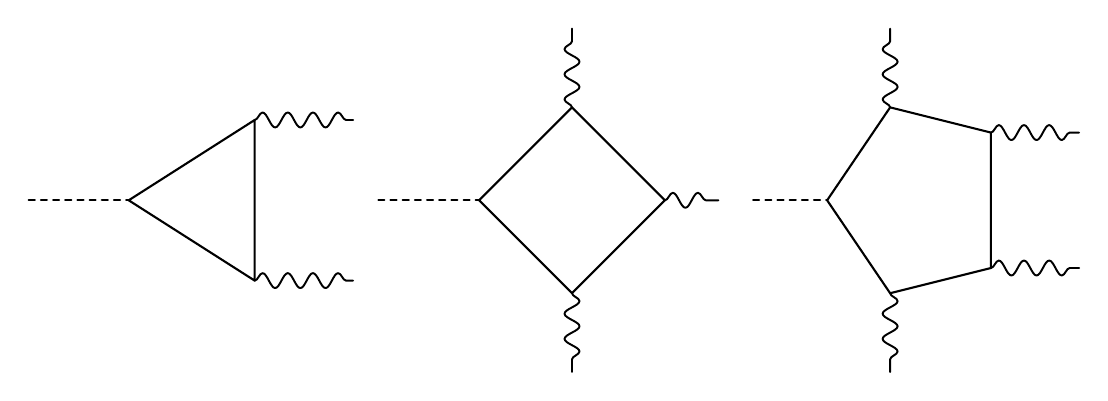
\begin{tikzpicture}[x=1cm,y=1cm,line cap=round,line join=round]
  \tikzset{
   fermion/.style={line width=0.76pt},
   current/.style={line width=0.75pt,dash pattern=on 2.2pt off 2.2pt},
   gauge/.style={
    line width=0.70pt,
    decorate,
    decoration={snake,amplitude=0.095cm,segment length=0.32cm}
   }
  }

  % Triangle.
  \coordinate (TL) at (-5.45,0);
  \coordinate (TU) at (-3.85,1.02);
  \coordinate (TD) at (-3.85,-1.02);
  \draw[current] (-6.72,0) -- (TL);
  \draw[fermion] (TL) -- (TU) -- (TD) -- cycle;
  \draw[gauge] (TU) -- (-2.60,1.02);
  \draw[gauge] (TD) -- (-2.60,-1.02);

  % Square.
  \coordinate (SL) at (-1.00,0);
  \coordinate (SU) at (0.18,1.18);
  \coordinate (SR) at (1.36,0);
  \coordinate (SD) at (0.18,-1.18);
  \draw[current] (-2.28,0) -- (SL);
  \draw[fermion] (SL) -- (SU) -- (SR) -- (SD) -- cycle;
  \draw[gauge] (SU) -- (0.18,2.18);
  \draw[gauge] (SR) -- (2.04,0);
  \draw[gauge] (SD) -- (0.18,-2.18);

  % Pentagon.
  \coordinate (PL) at (3.42,0);
  \coordinate (PUL) at (4.22,1.18);
  \coordinate (PUR) at (5.50,0.86);
  \coordinate (PDR) at (5.50,-0.86);
  \coordinate (PDL) at (4.22,-1.18);
  \draw[current] (2.48,0) -- (PL);
  \draw[fermion] (PL) -- (PUL) -- (PUR) -- (PDR) -- (PDL) -- cycle;
  \draw[gauge] (PUL) -- (4.22,2.18);
  \draw[gauge] (PUR) -- (6.62,0.86);
  \draw[gauge] (PDR) -- (6.62,-0.86);
  \draw[gauge] (PDL) -- (4.22,-2.18);
 \end{tikzpicture}
 \renewcommand{\thefigure}{22.2}
 \caption{One-loop diagrams for the anomaly in a current indicated by the
 dashed line. Solid lines are fermions; wavy lines are gauge fields with
 which they interact.}
 \label{fig:22.2}
\end{figure}


More specifically, in \hyperref[sec:22.2]{Section 22.2} we calculated the
divergence of an axial-vector current $J_5^\mu$, with
$t^L=-t^R\equiv t$, due to gauge-field interactions with vector currents
$J_\beta^\nu$ and $J_\gamma^\rho$ (called $J_\alpha^\nu$ and
$J_\beta^\rho$ in Section 22.2) with
$t_\beta^L=t_\beta^R\equiv t_\beta$, and likewise for $t_\gamma$. Hence in
this case $D_{\alpha\beta\gamma}$ is replaced with
$\operatorname{tr}[\{t,t_\beta\}t_\gamma]
=\operatorname{tr}[\{t_\beta,t_\gamma\}t]$, and Eq.~\eqref{eq:22.3.27}
becomes
\begin{equation}
 \left[
  \partial_\mu\bigl\langle J_5^\mu(x)\bigr\rangle
 \right]_{\mathrm{anom}}
 =-\frac{1}{32\pi^2}
 \operatorname{tr}[\{t_\beta,t_\gamma\}t]\,
 \epsilon^{\kappa\nu\lambda\rho}
 F_{\kappa\nu}^\beta(x)F_{\lambda\rho}^\gamma(x),
 \tag{22.3.29}\label{eq:22.3.29}
\end{equation}
in agreement with Eq.~\eqref{eq:22.2.26}.

Where no gauge fields are coupled to any of the currents
$J_\alpha^\mu(x)$, $J_\beta^\nu(y)$, or $J_\gamma^\rho(z)$, the choice of
the shift vector $a^\mu$ is a matter of convenience. When some but not all
currents are associated with symmetries that are spontaneously broken, we
keep the unbroken symmetries manifest if we choose $a^\mu$ so that there
are no anomalies in the currents corresponding to the unbroken symmetries.
(This will be important in \hyperref[sec:22.7]{Section 22.7}.) For instance,
in quantum chromodynamics and similar theories, where the generators
$T_\alpha$ of global symmetries like chiral $SU(3)\times SU(3)$ take the
form \eqref{eq:22.3.4}, all currents are either vector, with
$t_\alpha^R=t_\alpha^L$, corresponding to unbroken symmetries, or
axial-vector, with $t_\alpha^R=-t_\alpha^L$, corresponding to broken
symmetries. We see from Eq.~\eqref{eq:22.3.28} that in this case the only
triangle graphs with anomalies are those with one axial-vector and two
vector currents, or three axial-vector currents. In the case of one
axial-vector and two vector currents, we choose $a^\mu$ so that there is no
anomaly that interferes with the conservation of the vector currents. Thus,
if $J_\alpha^\mu(x)$ is the axial-vector current and $J_\beta^\nu(y)$ and
$J_\gamma^\rho(z)$ the two vector currents, then as in
Eq.~\eqref{eq:22.3.23} we must take $a^\mu=k_1^\mu-k_2^\mu$, so that the
anomaly is given by Eq.~\eqref{eq:22.3.24}. On the other hand, for three
axial-vector currents, there is no reason to require that any one of them
should be free of anomalies. Instead, it is natural to give $a^\mu$ a value
that respects the symmetry among the three currents. Guided by Lorentz
invariance, suppose we try $a=\alpha k_1+\beta k_2$, where $\alpha$ and
$\beta$ are constants.

Then symmetry would require that the momentum of \emph{each} internal line
should be $p$ plus $\alpha$ times the momentum flowing out at the end of the
line plus $\beta$ times the momentum flowing out at the beginning of the
line. That is, if we require that $a=\alpha k_1+\beta k_2$, then symmetry
requires also that
$a-k_1=-\alpha(k_1+k_2)+\beta k_1$ and
$a-k_2=\alpha k_2-\beta(k_1+k_2)$. These three relations are satisfied for
non-parallel $k_1$ and $k_2$ if and only if
$\alpha=-\beta=1/3$, so that
\begin{equation}
 a=\frac13(k_1-k_2).
 \tag{22.3.30}\label{eq:22.3.30}
\end{equation}
Using this in Eq.~\eqref{eq:22.3.22} and comparing with
Eq.~\eqref{eq:22.3.23}, we see that the anomaly in the axial-vector current
in a Feynman amplitude for three axial-vector currents is one-third what it
would be for one axial-vector and two vector currents.

The divergence of the current contains additional anomalies from the graphs
of Figure~\ref{fig:22.2}. Gauge invariance is no guide here, because even
the triangle graph does not yield conserved currents. The total anomaly has
been calculated by Bardeen~\hyperref[ch22-ref-8]{[8]} for the chiral
$SU(3)\times SU(3)$ symmetry of the strong interactions, with momentum shift
vectors chosen so that vector currents are conserved and graphs with all
axial currents are symmetric among these currents. Although this
$SU(3)\times SU(3)$ symmetry (which acts on quark flavors rather than colors)
is not gauged in quantum chromodynamics, it is convenient to express the
anomaly as a failure of gauge invariance in a functional $\Gamma[V,A]$ of
fictitious weakly coupled gauge fields: an octet of vector fields
$V_a^\mu(x)$ and an octet of axial-vector fields $A_a^\mu(x)$. We also
introduce infinitesimal gauge-transformation operators\footnote{The
operators $\mathcal V_a$ and $\mathcal A_a$ here are what in
Ref.~\hyperref[ch22-ref-8]{[8]} were called $X_a$ and $Y_a$. This switch in
notation is made to maintain consistency with the notation of Chapter 19,
where broken symmetry generators are consistently labelled $X_a$.}
\begin{equation}
 \begin{aligned}
 i\mathcal V_a(x)
 ={}&-\frac{\partial}{\partial x^\mu}
 \frac{\delta}{\delta V_{a\mu}(x)}
 -f_{abc}V_{b\mu}(x)\frac{\delta}{\delta V_{c\mu}(x)}
 -f_{abc}A_{b\mu}(x)\frac{\delta}{\delta A_{c\mu}(x)}
 \end{aligned}
 \tag{22.3.31}\label{eq:22.3.31}
\end{equation}
and
\begin{equation}
 \begin{aligned}
 i\mathcal A_a(x)
 ={}&-\frac{\partial}{\partial x^\mu}
 \frac{\delta}{\delta A_{a\mu}(x)}
 -f_{abc}V_{b\mu}(x)\frac{\delta}{\delta A_{c\mu}(x)}
 -f_{abc}A_{b\mu}(x)\frac{\delta}{\delta V_{c\mu}(x)},
 \end{aligned}
 \tag{22.3.32}\label{eq:22.3.32}
\end{equation}
where $f_{abc}$ are the $SU(3)$ structure constants. As mentioned above,
the labelling of internal line momenta is chosen so that the vector current
is not anomalous:
\begin{equation}
 \mathcal V_a\Gamma[V,A]=0,
 \tag{22.3.33}\label{eq:22.3.33}
\end{equation}
but then an anomaly appears in the axial-vector currents
\begin{equation}
 \begin{aligned}
 \mathcal A_a\Gamma[V,A]
 =\frac{i}{32\pi^2}\epsilon^{\mu\nu\rho\sigma}
 \operatorname{Tr}\Biggl\{\lambda_a\Biggl[
 &V_{\mu\nu}V_{\rho\sigma}
 +\frac13A_{\mu\nu}A_{\rho\sigma}
 -\frac{32}{3}A_\mu A_\nu A_\rho A_\sigma
 \\
 &+\frac{8i}{3}\left(
  A_\mu A_\nu V_{\rho\sigma}
  +A_\mu V_{\rho\sigma}A_\nu
  +V_{\rho\sigma}A_\mu A_\nu
 \right)
 \Biggr]\Biggr\}.
 \end{aligned}
 \tag{22.3.34}\label{eq:22.3.34}
\end{equation}

where $\lambda_a$ are the $SU(3)$ matrices given by
Eq.~\eqref{eq:19.7.2}, and
\begin{equation}
 V_\mu\equiv\frac12\lambda_a V_{\mu a},
 \qquad
 A_\mu\equiv\frac12\lambda_a A_{\mu a},
 \tag{22.3.35}\label{eq:22.3.35}
\end{equation}
\begin{equation}
 V_{\mu\nu}
 =\partial_\mu V_\nu-\partial_\nu V_\mu
 -i[V_\mu,V_\nu]-i[A_\mu,A_\nu],
 \tag{22.3.36}\label{eq:22.3.36}
\end{equation}
\begin{equation}
 A_{\mu\nu}
 =\partial_\mu A_\nu-\partial_\nu A_\mu
 -i[V_\mu,A_\nu]-i[A_\mu,V_\nu].
 \tag{22.3.37}\label{eq:22.3.37}
\end{equation}
The factor $1/3$ accompanying the second term on the right-hand side in
Eq.~\eqref{eq:22.3.34} has already been explained as a consequence of the
different choice of $a^\mu$ in the $AVV$ and $AAA$ graphs. In
\hyperref[sec:22.6]{Section 22.6} we will describe consistency conditions
that allow the cubic and quartic terms in Eq.~\eqref{eq:22.3.34} to be
calculated from the quadratic terms.

For anomalies involving symmetries that are \emph{all} spontaneously
broken, there is no reason to choose $a^\mu$ in a way that distinguishes
among the different currents, and instead it is natural to label internal
fermion lines in a way that is symmetric among the attached gauge boson
lines. As we have seen, this means that the triangle graph is to be
calculated with the choice $a=\frac13(k_1-k_2)$. This gives a triangle
anomaly one-third of the value given by \eqref{eq:22.3.26}. When square and
pentagon graphs are included, this result becomes
\hyperref[ch22-ref-8a]{[8a]}
\begin{equation}
 \begin{aligned}
 \bigl[(D_\mu J_\alpha^\mu)\bigr]_{\mathrm{anom}}
 =-\frac{1}{24\pi^2}\epsilon^{\kappa\nu\lambda\rho}
 \operatorname{Tr}\Bigl\{T_\alpha\bigl[
 &\partial_\kappa A_\nu\,\partial_\lambda A_\rho
 -\frac{i}{2}\partial_\kappa A_\nu A_\lambda A_\rho
 \\
 &+\frac{i}{2}A_\kappa\partial_\nu A_\lambda A_\rho
 -\frac{i}{2}A_\kappa A_\nu\partial_\lambda A_\rho
 \bigr]\Bigr\},
 \end{aligned}
 \tag{22.3.38}\label{eq:22.3.38}
\end{equation}
where $A^\mu\equiv A_\alpha^\mu T_\alpha$. We will not derive this result
here, because we have already seen that in such cases the terms quadratic
in $A_\mu$ are given by one-third the corresponding terms in
Eq.~\eqref{eq:22.3.26}, and in \hyperref[sec:22.6]{Section 22.6} we shall
be able to use consistency conditions to derive the remaining terms in
Eq.~\eqref{eq:22.3.38} from the quadratic terms.

Now we must consider possible corrections to these results. A careful
derivation of the anomaly to all orders of perturbation theory was given by
Adler and Bardeen~\hyperref[ch22-ref-9]{[9]}; what follows is intended to
give only the gist of their analysis.

The argument that led to Eq.~\eqref{eq:22.3.22} may be repeated in any
order of perturbation theory, and shows that the anomaly in general arises
from momentum-space integrals that can be reexpressed as surface terms. In
consequence, as we saw here in Eq.~\eqref{eq:22.3.18}, the only graphs for
the current divergence that contribute to the anomaly are those for which
the integral over the momentum circulating in the fermion loop has
dimensionality (in powers of momentum) zero or greater. Interactions of the
fermions in the loop with virtual gauge bosons would reduce the
dimensionality of the integral over the fermion loop momentum enough to
eliminate the anomaly, so the anomaly receives no contribution from such
radiative corrections. (It is true that the integral over the momenta of
the virtual gauge bosons as well as the fermion loop would have
non-negative dimensionality, but the gauge boson propagators can be
regulated, as the fermion propagator cannot, without interfering with the
chiral symmetry in question.) The anomaly is affected by interactions of
the gauge bosons attached to the fermion loop with other gauge bosons and
fermion loops, but these just serve to renormalize operators like
$\epsilon^{\kappa\nu\lambda\rho}F_{\kappa\nu}^{\beta}(x)
F_{\lambda\rho}^{\gamma}(x)$. By the same argument, any fermion mass that
respects the symmetries in question (if this were possible) would not
change the anomaly, because extracting factors of this mass would lower
the dimensionality of the momentum-space integral.

The last remark of the previous paragraph raises the question of whether
we can calculate the anomaly without knowing all the fermions in a theory,
heavy fermions as well as light or massless ones. Yes, we can; we shall now
show that \emph{no fermion that is allowed by a given symmetry to have a
mass can contribute to the anomaly for that symmetry}. In the general
class of theories considered here, a mass term in the Lagrangian density
would take the form
\begin{equation}
 \mathcal L_{\mathrm{mass}}
 =-\sum_{nn'\sigma\sigma'}
 \chi_{\sigma n}\epsilon_{\sigma\sigma'}M_{nn'}\chi_{\sigma'n'}
 +\mathrm{H.c.},
 \tag{22.3.39}\label{eq:22.3.39}
\end{equation}
where $\sigma$ is the two-component spinor index of the $(1/2,0)$
representation of the Lorentz group, $\epsilon_{\sigma\sigma'}$ is the
antisymmetric matrix with $\epsilon_{1/2,-1/2}=+1$, needed for Lorentz
invariance, and $M$ is a symmetric mass matrix.\footnote{In
fermion-number-conserving theories where $\chi$ has the form
\eqref{eq:22.3.1}, $M$ is related to the usual mass matrix $m$ by
\[
 M=\frac12
 \begin{pmatrix}
  0&m\\
  m^{\mathsf T}&0
 \end{pmatrix}.
\]
With all inversion phases equal to unity, parity, charge conjugation, and
time-reversal invariance respectively have the further consequences that
$m$ is Hermitian, symmetric, or real.} Now, in order for
$\mathcal L_{\mathrm{mass}}$ to respect gauge invariance, the mass matrix
must satisfy
\begin{equation}
 -T_\alpha^{\mathsf T}M=MT_\alpha.
 \tag{22.3.40}\label{eq:22.3.40}
\end{equation}
The index $n$ may be replaced with an index $r$ labelling different
irreducible representations of the gauge group, and an index $s$ labelling
components within each irreducible representation, so that
\begin{equation}
 (T_\alpha)_{rs,r's'}=\delta_{rr'}(T_\alpha^{(r)})_{s,s'},
 \tag{22.3.41}\label{eq:22.3.41}
\end{equation}
and we write
\begin{equation}
 M_{rs,r's'}=(M^{(r,r')})_{ss'}.
 \tag{22.3.42}\label{eq:22.3.42}
\end{equation}
Equation~\eqref{eq:22.3.40} then becomes
\begin{equation}
 -T_\alpha^{(r)\mathrm T}M^{(r,r')}
 =M^{(r,r')}T_\alpha^{(r')}.
 \tag{22.3.43}\label{eq:22.3.43}
\end{equation}
(This is not summed over $r$ or $r'$.) Schur's
lemma~\hyperref[ch22-ref-10]{[10]} tells us that whenever the matrices of a
pair of irreducible representations are related by such an equation, the
matrix that relates them is either zero or non-singular. (See
\hyperref[sec:5.5]{Section 5.5}.) Thus, either (i) $M^{(r,r')}=0$, or else
(ii) $-T_\alpha^{(r)\mathrm T}$ and $T_\alpha^{(r')}$ are related by a
similarity transformation, and likewise for $T_\beta$ and $T_\gamma$. In
the latter case the contributions to the anomaly constant
\eqref{eq:22.3.12} from fermions belonging to the individual irreducible
representations $r$ and $r'$ are related by
\begin{equation}
 D_{\alpha\beta\gamma}^{(r)}
 =-D_{\alpha\beta\gamma}^{(r')},
 \tag{22.3.44}\label{eq:22.3.44}
\end{equation}
so the anomaly either vanishes (for $r=r'$) or cancels between the two
representations (for $r\ne r'$). The anomalies in a given set of
symmetries therefore are unaffected by the possible presence of fermions
with a mass allowed by these symmetries.

\begin{center}
 $\ast\qquad\ast\qquad\ast$
\end{center}

There is a fine point in the use of the Feynman rules to calculate the
three-point function \eqref{eq:22.3.7}, to which we now return. In using the
conventional fermion propagator \eqref{eq:22.3.9}, we have in effect
doubled the number of fermion fields; in additional to the purely
left-handed fields $\chi(x)$ given by Eq.~\eqref{eq:22.3.1}, the propagator
\eqref{eq:22.3.9} includes right-handed modes (unrelated to the fields
$(1-\gamma_5)\psi$ of fermion-number-conserving theories) that do not
interact with the gauge fields. Combining these non-interacting
right-handed fields with the interacting left-handed fields in a single
spinor $\Psi$, the fermion Lagrangian density is
$-\overline\Psi\sl{D}\Psi$, where $\sl{D}$ is now
\begin{equation}
 \sl{D}=\sl{\partial}
 -iA_\alpha T_\alpha\left(\frac{1+\gamma_5}{2}\right).
 \tag{22.3.45}\label{eq:22.3.45}
\end{equation}

The one-loop vacuum functional for spin $1/2$ fields interacting with real
or fictitious gauge fields is just $\operatorname{Det}\sl{D}$. The failure
of gauge invariance in this determinant can be blamed on the fact that the
operator \eqref{eq:22.3.45} is the sum of two terms
\begin{equation}
 \sl{D}
 =\sl{\partial}\left(\frac{1-\gamma_5}{2}\right)
 +\sl{D}\left(\frac{1+\gamma_5}{2}\right),
 \tag{22.3.46}\label{eq:22.3.46}
\end{equation}
of which only the second is gauge-invariant.

There is another way of looking at anomalies
\hyperref[ch22-ref-10a]{[10a]}, which provides a framework for calculations
of a large class of anomalies, of coordinate as well as gauge symmetries
in spaces of any dimensionality. Instead of working with the operator
\eqref{eq:22.3.45}, which has a well-defined determinant, one deals instead
with just the second term in Eq.~\eqref{eq:22.3.46}
\begin{equation}
 \sl{D}_L=\sl{D}\left(\frac{1+\gamma_5}{2}\right).
 \tag{22.3.47}\label{eq:22.3.47}
\end{equation}
This is perfectly gauge-invariant, but does not have a well-defined
determinant, because this operator does not map the space of fermion fields
of one handedness into itself, but rather into the space of fermion fields
of the other handedness. One can try to define a gauge-invariant vacuum
functional $\operatorname{Det}\sl{D}_L$ by writing differential equations
for $\operatorname{Det}\sl{D}_L$ in the space of gauge fields, modulo gauge
transformations, but then one may encounter obstructions. There are local
obstructions due to violations of the necessary integrability conditions,
which correspond to the anomalies we have been discussing. Even where
these local obstructions are absent, in cases where the
infinite-dimensional space of gauge-field configurations, modulo gauge
transformations, is not simply connected, topological obstructions can
prevent the definition of single-valued functionals on this space. Such a
global anomaly was found by Witten~\hyperref[ch22-ref-10b]{[10b]} for the
gauge group $SU(2)$ (which is free of local anomalies) with an odd number
of massless left-handed fermions in $SU(2)$ doublets.
